%%% Template originaly created by Karol Kozioł (mail@karol-koziol.net) and modified for ShareLaTeX use

\documentclass[a4paper,11pt]{article}
\usepackage[russian]{babel}
\usepackage[T1]{fontenc}
\usepackage[utf8]{inputenc}
\usepackage{graphicx}
\usepackage{xcolor}
\usepackage{amsmath}
\usepackage{amssymb}
\renewcommand\familydefault{\sfdefault}
\usepackage{tgheros}
\newcommand*{\Perm}[2]{{}^{#1}\!P_{#2}}%
\newcommand*{\Comb}[2]{{}^{#1}C_{#2}}%
\usepackage{amsmath,amssymb,amsthm,textcomp}
\usepackage{enumerate}
\usepackage{multicol}
\usepackage{tikz}
\usepackage{graphicx}

\usepackage{geometry}
\geometry{left=25mm,right=25mm,%
bindingoffset=0mm, top=20mm,bottom=20mm}


\linespread{1.3}

\newcommand{\linia}{\rule{\linewidth}{0.5pt}}

% custom theorems if needed
\newtheoremstyle{mytheor}
    {1ex}{1ex}{\normalfont}{0pt}{\scshape}{.}{1ex}
    {{\thmname{#1 }}{\thmnumber{#2}}{\thmnote{ (#3)}}}

\theoremstyle{mytheor}
\newtheorem{defi}{Definition}

% my own titles
\makeatletter
\renewcommand{\maketitle}{
\begin{center}
\vspace{2ex}
{\huge \textsc{\@title}}
\vspace{1ex}
\\
\linia\\
\@author \hfill \@date
\vspace{4ex}
\end{center}
}
\makeatother
%%%

% custom footers and headers
\usepackage{fancyhdr}
\pagestyle{fancy}
\lhead{}
\chead{}
\rhead{}
%\lfoot{Assignment \textnumero{} 5}
\cfoot{}
\rfoot{Page \thepage}
\renewcommand{\headrulewidth}{0pt}
\renewcommand{\footrulewidth}{0pt}
%

% code listing settings
\usepackage{listings}
\lstset{
    language=Python,
    basicstyle=\ttfamily\small,
    aboveskip={1.0\baselineskip},
    belowskip={1.0\baselineskip},
    columns=fixed,
    extendedchars=true,
    breaklines=true,
    tabsize=4,
    prebreak=\raisebox{0ex}[0ex][0ex]{\ensuremath{\hookleftarrow}},
    frame=lines,
    showtabs=false,
    showspaces=false,
    showstringspaces=false,
    keywordstyle=\color[rgb]{0.627,0.126,0.941},
    commentstyle=\color[rgb]{0.133,0.545,0.133},
    stringstyle=\color[rgb]{01,0,0},
    numbers=left,
    numberstyle=\small,
    stepnumber=1,
    numbersep=10pt,
    captionpos=t,
    escapeinside={\%*}{*)}
}

%%%----------%%%----------%%%----------%%%----------%%%

\begin{document}

\title{Типовой расчёт \textnumero{} 4}

\author{Анужин Баатарцогт, M3112}

\date{05/15/2020}

\maketitle

\section*{Задание 1}
(1 балл) Возьмём все перестановки из пяти чисел. В скольких из них ни одно число не стоит на своём месте?
\newline
\section*{Решение:}
n - количество всего элементов, r - число элементов стояших на месте, n-r - число перемешений \\
$N^{(r)} = C_n^r  P_(n-r)$  \\
$N^{(0)} = P_5 - C_5^1P_4 + C_5^2P_3 - C_5^3P_2 + C_5^4P_1 - C_5^5P_0$
$ = 120 -5*24 + 10*6 - 10*2 + 5*1 - 1*1 = 44$\\ \\
\textbf{Ответ :} 44 случая\\


\section*{Задание 2}

(1 балл) Я хочу послать своему другу 8 фотографий. Сколькими способами можно разложить их по 5-ти конвертам ?
\newline
\section*{Решение:}
\textbf{Каждая фотография может находиться 1-5 кармане, то есть} \\
\textbf{$5 \times 5 \times 5 \times 5 \times 5 \times 5 \times 5 \times 5  = 5^8$}

\newline

\section*{Задание 3}
(1 балл) У скольких натуральных чисел меньше 10000, сумма равна 10?.
\section*{Решение:}
Разбим числа на части 0-99, 100-999, 1000-9999. N - число способов.\\
1. При 0 - 99 : 19, 28, 37, 46, 55, 64, 73, 82, 91.\\
$$N_1 = 9$$
\newline
2. При 100 - 999: \\
1(0-9)(9-0), N = 10 \\
2(0-8)(8-0), N = 9  \\
3(0-7)(7-0), N = 8  \\
... \\
9(0-1)(1-0),  N = 2  \\
$$N_2 = \sum_{n=1}^{10} n = 54$$ 
\newline
3. При 1000-9999: \\
10(0-9)(9-0), N = 10  \\
11(0-8)(8-0), N = 9 \\
12(0-7)(7-0), N = 8  \\
... \\
20(0-8)(8-0), N = 9 \\ 
21(0-7)(7-0), N = 8 \\ 
22(0-6)(6-9), N = 7 \\ 
...\\
30(0-7)(7-0), N = 8  \\ 
31(0-6)(6-0), N =  7  \\ 
32(0-5)(5-0), N =  6  \\ 
Итак видно что числа способов уменьшивается на 1 при возрастений числа\\.  
$$N_3 = \sum_{n=1}^{10} n + \sum_{n=1}^{9} n + \sum_{n=1}^{8} n + \sum_{n=1}^{7} n + \sum_{n=1}^{6} n + \sum_{n=1}^{5} n + \sum_{n=1}^{4} n + \sum_{n=1}^{3} n + \sum_{n=1}^{2} n = 219$$	

\vspace{0.5 cm}

\textbf{N = N_1 + N_2 + N_3 = 9 + 54 + 219 = 282}\newline

\textbf{\Lareg{Ответ :} 282}

\section*{Задание 4}
(1 балл) Сколькими способами можно разбить 14 человек на пары?
\newline
\section*{Решение:}
\large $N = \frac{C_{14}^{2} \times C_{12}^{2} \times C_{10}^{2} \times C_{8}^{2} ... \times C_{2}^{2}}{7!} = 135135$\newline
\textbf{\Lareg{Ответ :} 135135}

\section*{Задание 5}

\includegraphics[width=\textwidth,height=\textheight,keepaspectratio]{image.png} \newline
(2 балла) Для представленного графа определите:\newline
1. есть ли в графе Эйлеров цикл или Эйлерова цепь? Если
есть, то выпишите. Если нет, то обоснуйте отсутствие;
\newline

\section*{Решение:}
\newline
\large{В этом графе нет Эйлеров цикла. Потому что граф имеет эйлерова
цикл если вершины имеет чётную степень и находитса в одном компоненте связности. В этом графе вершины a-j имеют нечетную степень 3, зато они находится в одном компоненте связности.}
\newline
\lareg{ В этом графе нет Эйлерова цепь. В неориентированном графе есть эйлеровый цепь если граф связной и количество вершин с нечётной степенью равен 0 или 2. В нашем графе  количество вершин с нечетной степенью равно 10.\\}
\newline \\
2. Есть ли в графе Гамильтонов цикл, Гамильтонова цепь?
Если есть, то выпишите. Если нет, то обоснуйте отсутствие;
\newline
\section*{Решение:}
\large{ Цикл - это просто ребро, соединяющее вершину с самим собой; таким образом, гамильтонов цикл - это путь, идущий от вершины к себе, посещающий каждую вершину в пути один раз.\\
В  нашем графе существует Гамильтонова цикл $A\Rightarrow B\Rightarrow C\Rightarrow D\Rightarrow J\Rightarrow F \Rightarrow G\Rightarrow H\Rightarrow I\Rightarrow E \Rightarrow A $
}
\newline
\lareg{ В графе есть Гамильтонова цепь : $A\Rightarrow B\Rightarrow C\Rightarrow D\Rightarrow E\Rightarrow I \Rightarrow  H\Rightarrow G\Rightarrow F \Rightarrow J $\newline
\section*{Задание 6}
(1 балл) Нарисуйте дерево с диаметром 7, причем вершин центра должна быть 2, а листьев не менее 8.
\section*{Решение:}
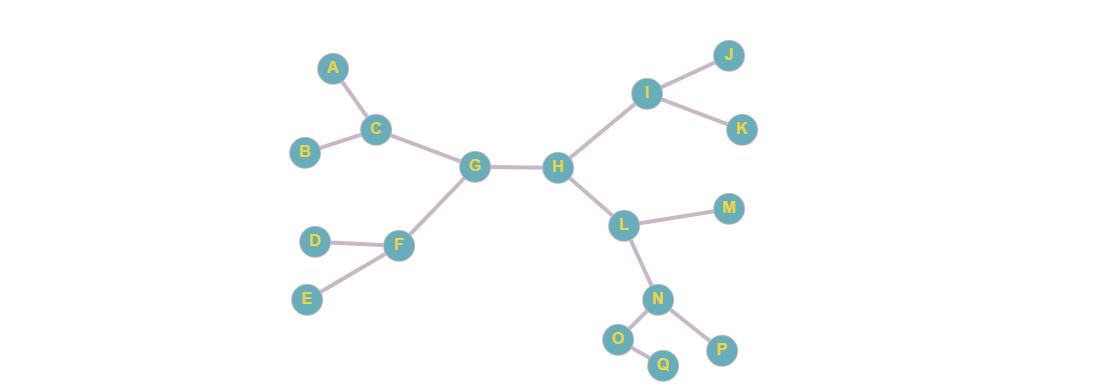
\includegraphics[width=\textwidth,height=\textheight,keepaspectratio]{download.png}
\large{ Центры H, L. Диаметр равен 7 ${A \Rightarrow C \Rightarrow G \Rightarrow H \Rightarrow L \Rightarrow N \Rightarrow O \Rightarrow Q }$
\hfill \hfill

\section*{Задание 7}
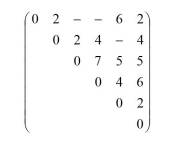
\includegraphics[width=120,height=120]{7.PNG}\newline

(3 балла) Граф задан матрицей расстояний. Требуется:\newline
1. построить минимальное остовное дерево;\newline
2. построить фундаментальную систему циклов, ассоциированную с этим остовом;\newline
3. найти кратчайшие пути от вершины 4 до всех остальных вершин графа.\newline

\section*{Решение:}
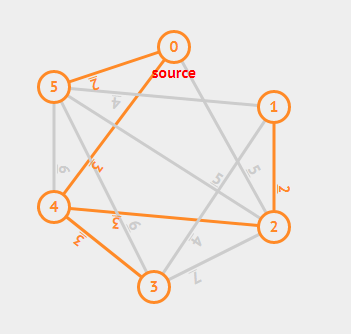
\includegraphics[width=150,height=150]{kruskal.PNG}\newline
1. Вес минимального остовного дерева равен 13.\newline
\Lareg{{2. Фундаментальная система циклов:}}\newline
Фундаментальный цикл графа G относительно остова T  — простой цикл C, полученный путем добавления к остову T ребра {e1e2} \not \in T. \\

\includegraphics[width=\textwidth,height=\textheight,keepaspectratio]{cycle.png}\newline

\includegraphics[width=\textwidth,height=\textheight,keepaspectratio]{cycle2.png}\newline

\includegraphics[width=\textwidth,height=\textheight,keepaspectratio]{cycle3.png}\newline 

3.\Lareg{{Найти кратчайшие пути от вершины 4 до всех остальных вершин графа.}}\newline
$4\Rightarrow 0 : d = 3$\newline
$4\Rightarrow2 \Rightarrow 1: d = 3 + 2 = 5 $\newline
$4\Rightarrow2: d = 3 $\newline
$4\Rightarrow3: d = 3 $\newline
$4\Rightarrow 0 \Rightarrow 5: d = 3 + 2 = 5$\newline
\end{document}
